% Gemini theme
% https://github.com/anishathalye/gemini

\documentclass[final]{beamer}

% ====================
% Packages
% ====================

\usepackage[T1]{fontenc}
\usepackage{caption}
\usepackage{subcaption}
\usepackage[superscript,biblabel]{cite}
\usepackage{lmodern}
\usepackage[scale=1.15,size=a0,orientation=portrait]{beamerposter}
%\usepackage[size=custom,width=90,height=130,scale=1.25]{beamerposter}
\usetheme{gemini}
\usecolortheme{labsix}
\usepackage{graphicx}
\usepackage{svg}
\svgsetup{inkscapeexe=/Applications/Inkscape.app/Contents/MacOS/inkscape}
\DeclareGraphicsRule{.ai}{pdf}{.ai}{}
\usepackage{booktabs}
\usepackage[none]{hyphenat}
\usepackage{amsmath}
\usepackage{amssymb}
\usepackage{tikz}
\usetikzlibrary{fit,backgrounds}
\usepackage{pgfplots}
\usepgfplotslibrary{fillbetween}


% ====================
% Lengths
% ====================

% If you have N columns, choose \sepwidth and \colwidth such that
% (N+1)*\sepwidth + N*\colwidth = \paperwidth
\newlength{\sepwidth}
\newlength{\colwidth}
\setlength{\sepwidth}{0.025\paperwidth}
\setlength{\colwidth}{0.3\paperwidth}

\newcommand{\separatorcolumn}{\begin{column}{\sepwidth}\end{column}}

% ====================
% Title
% ====================

\title{Mesoscopic thermodynamics of single-particle enzymatic reactions}

% REMOVED \inst{1}
\author{Filipe P. de Farias\inst{1} \and Francesco Corona\inst{2}  \and Michela Mulas\inst{1}}

\institute[UFC]{\inst{1}Post-graduate Programme in Teleinformatics Engineering, Federal University of Ceará, Brazil\\ \inst{2}School of Chemical Engineering, Aalto University, Finland}

% ====================
% Footer (optional)
% ====================
 %% REMOVED {  %\href{https://www.example.com}{https://www.example.com} 
  %\href{mailto:alyssa.p.hacker@example.com}{alyssa.p.hacker@example.com} }
\footercontent{
  \hfill
  Challenges in the Physics of Active and Biological Matter 2023
  \hfill
}
% (can be left out to remove footer)

% ====================
% Logo (optional)
% ====================

% use this to include logos on the left and/or right side of the header:
\logoright{\includegraphics[height=10cm,
%page=2,trim={17cm 21cm 3cm 5cm},clip
]{"graphics/brasao2_vertical_monocromatico"}}
\logoleft{\includegraphics[height=10cm,trim={50 50 50 50},clip]{"graphics/logo-31148-1"}}

% ====================
% Body
% ====================

\begin{document}

\setlength{\abovedisplayskip}{40pt}
\setlength{\belowdisplayskip}{40pt}

\begin{frame}[t]
\begin{columns}[t]
\separatorcolumn

\begin{column}{\colwidth}

\begin{block}{Michaelis-Menten theory}
The Michaelis-Menten kinetics models the kinetics of enzyme $E$ reacting with substrate $S$ forming complex $ES$ which releases product $P$ and enzyme according to the following chemical reaction network: 
\begin{equation*}
E + S \underset{k_{-1}}{\stackrel{k_1}{\rightleftharpoons}} ES \underset{k_{-2}}{\stackrel{k_2}{\rightleftharpoons}} E + P.
\end{equation*}
%
In this analysis, it is assumed that:
\begin{itemize}
\justifying
\item The amounts of $S$ and $P$ are considered to be much larger than of $E$ and $ES$ such that a reaction does not change considerably the quantities of $S$ and $P$;
\item The reactions are modeled as random interactions of the enzyme with the reservoir in equilibrium at temperature T formed by the solution of $S$ and $P$\cite{Seifert:2010aa}.
\end{itemize}
%
\begin{figure}
\centering
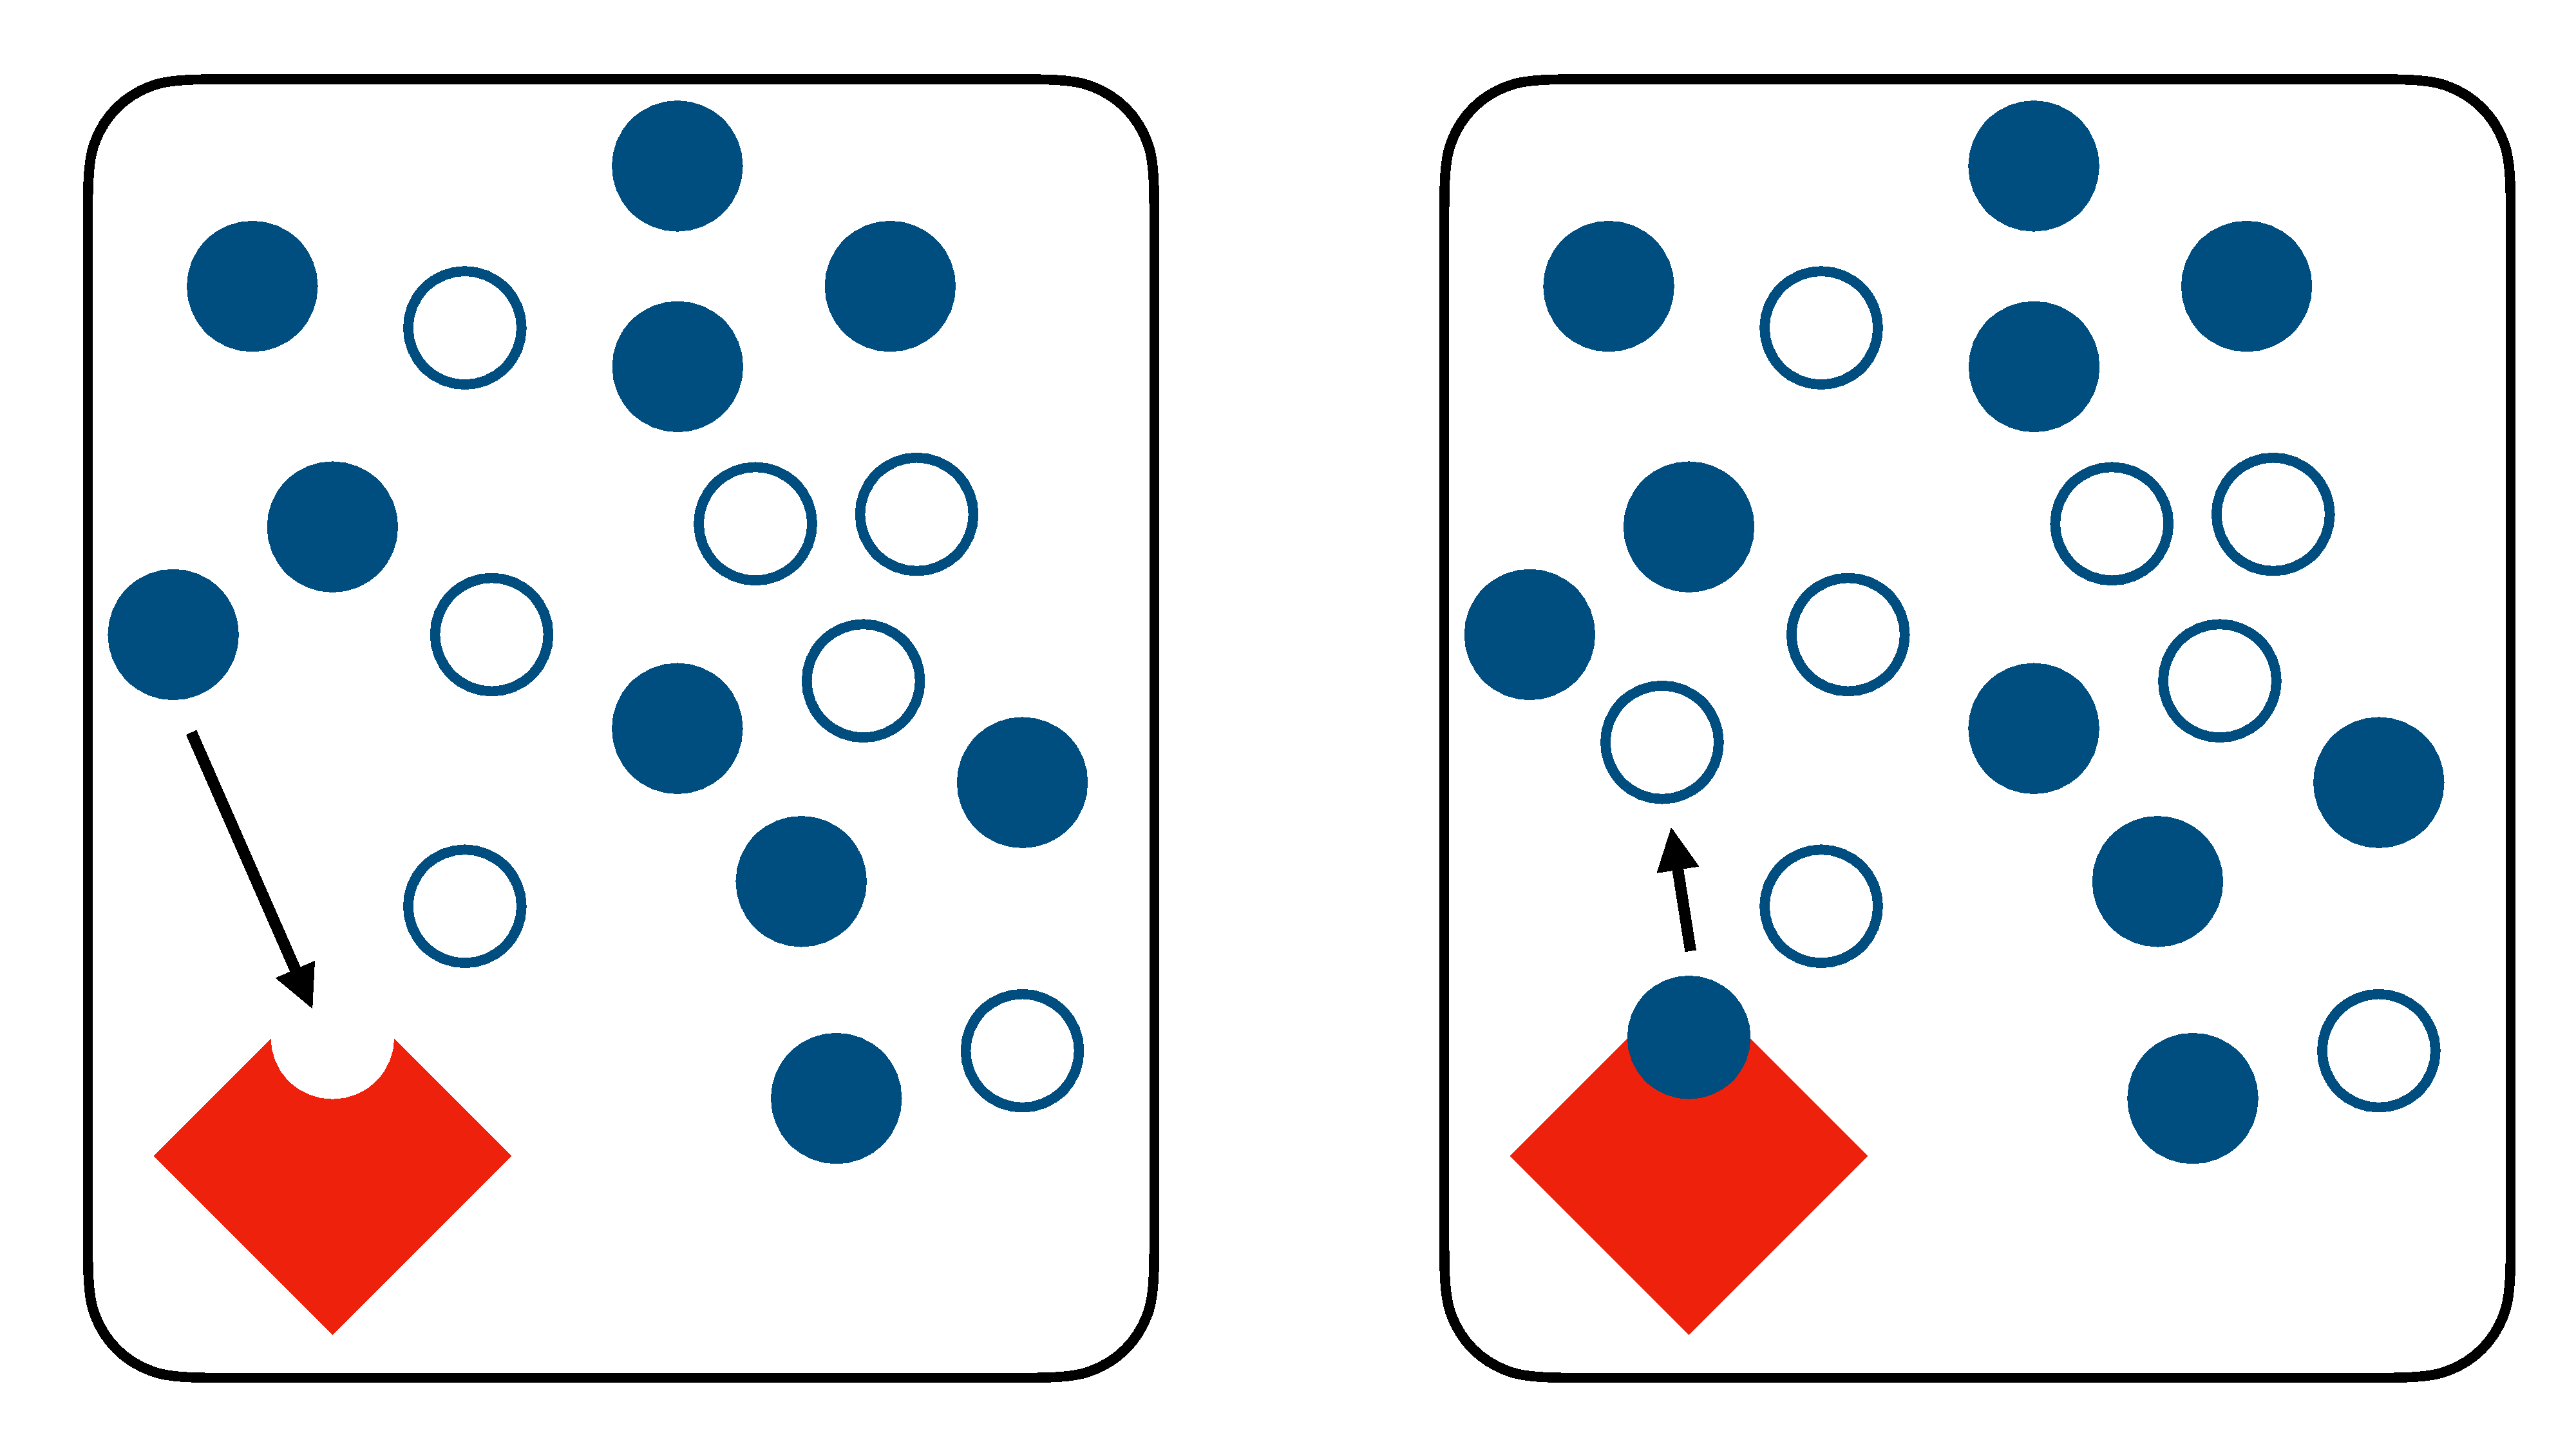
\includegraphics[width=.8\textwidth]{graphics/MichaelisMenten.pdf}
\caption{\justifying Figure adapted from Seifert (2010)\cite{Seifert:2010aa}, where the solution is composed by substrate (filled circle), product (empty circle) and single enzyme (red square). The single enzyme is interacting with the solution changing its state.}
\vskip-20pt
\end{figure}
%
The system considered for this analysis consists of $n_E$ molecules of $E$ and $n_{ES}$ molecules of $ES$, being the system states $\{ x \in \mathcal{X} | x = (x_i,x_{i^\prime}) \}$ with $ \mathcal{X} = \{0,...,n_E\}\!\times\! \{0,...,n_E\}$.

%Considering only one enzyme, the states in which it is found is $E$ or $ES$, thus the number of molecules of each of them are $n_E \in \{0,1\}$ and $n_{ES} \in \{0,1\}$, respectively.
\begin{itemize}
\justifying
%%
\item The evolution of the system is modeled as a Markov jump process between states $x$ whose probability $p_x(t)$ solves the following {\bf master equation}\cite{van2007stochastic,GILLESPIE1976403}
%
\begin{equation}
\frac{dp_{x}(t)}{dt} = \sum_{\mathcal{X}} W_{x^\prime x} p_{x}(t) -  W_{x x^\prime}p_{x^\prime}(t) \label{eq CME}
\end{equation}
%\item $W_{x x^\prime }(k_\nu)$ is the {\bf probability transition rate} from a state $x^\prime$ to state $x$, it depends on the kinetics, and it is an element of the $2 \times 2$ rate transition matrix $W$\cite{Munsky_2006}:
\item $W_{x x^\prime }(k_\nu)$ is the {\bf probability transition rate} from a state $x^\prime$ to state $x$, it depends on the kinetics, and it is an element of the $|\mathcal{X}|\times|\mathcal{X}|$ rate transition matrix $W$ equal to\cite{Munsky_2006}:
\begin{equation*}
-\sum_\nu a_\nu({x},k_\nu) \delta(x - x^\prime) + a_\nu({x} - s_\nu,k_\nu) \delta(x - x^\prime + s_\nu),
\end{equation*}
\vskip-20pt
where the following terms were defined:\\

- $a_\nu({x},k_\nu) = \prod_{x_i \in x} k_\nu \cfrac{{x_i}!}{({x}_{i} - s_{i,\nu})!}$ is the propensity function for the $\nu$-th reaction with rate $k_\nu$;\\

- $s_{i,\nu} $ is the change in the number of molecules of $x_i \in x$ participating in the $\nu$-th reaction;\\
- $\delta(x) = 1$ only if $x \equiv (0,0)$, otherwise is $0$.
%
\end{itemize}
%

Considering the system with $n_E=n_{ES}=1$, it can be verified that the states $(0,0)$ and $(1,1)$ have no transitions coming to or leaving them, thus $W$ can be reduced to $2 \times 2$ and set $p_x(t) = 0$ for those states. 
\end{block}


\begin{alertblock}{References}

%\nocite{*}
\footnotesize{\bibliographystyle{plain}\bibliography{poster-Phys-ActBio-Matter-2023}}

\end{alertblock}
\end{column}

\separatorcolumn

\begin{column}{\colwidth}

\begin{block}{Stochastic Thermodynamics (ST)}
\vskip10pt
\justifying
The energy transfer in systems modeled at the mesoscopic scale with stochastic dynamics which are open and out-of-equilibrium is the subject of Stochastic Thermodynamics\cite{peliti2021stochastic,Falasco:2023aa}. 
%
\begin{itemize}
\justifying
\item Systems at equilibrium are {\bf reversible}, i.e. the transition $x \rightarrow x^\prime$ occurs with rate $W_{xx^\prime}$, and its reversed transition $x^\prime \rightarrow x$ has the rate $W_{x^\prime x}=W_{xx^\prime}$.

\item At {\bf nonequilibrium} a system is kept at steady-state by exchanging an entropy to the reservoir (local detailed balance, LDB) which is proportional to $\ln (W_{xx^\prime} / W_{x^\prime x})$\cite{10.21468/SciPostPhysLectNotes.32}.
\end{itemize}
\begin{itemize}
\justifying
\item The transition $x^\prime \rightarrow x$ exchanges with the reservoir an amount of entropy equal to
%
\begin{equation}
s^{flu}_{x^\prime \rightarrow x} = k_B T \ln \frac{W_{xx^\prime}}{W_{x^\prime x}}.
\label{eq stoch ent res}
\end{equation}
%
\item In the same transition, the system produces an amount of entropy equal to
%
\begin{equation*}
s^{prod}_{x^\prime \rightarrow x} = k_B T \ln \frac{W_{xx^\prime}p_{x^\prime}(t)}{W_{x^\prime x}p_x(t)}.
\label{eq stoch ent prod}
\end{equation*}
%
\item The entropy balance during the transition is
%
\begin{equation*}
s^{bal}_{x^\prime \rightarrow x} = k_B T \ln \frac{p_x^\prime(t)}{p_x(t)}.
\label{eq stoch ent bal}
\end{equation*}
%
which is equal to $s^{prod}_{x^\prime \rightarrow x} - s^{flu}_{x^\prime \rightarrow x}$.
\end{itemize}
The average of \eqref{eq stoch ent res} over the probability of the system to transition to $x$ gives the {\bf average entropy flux rate}\cite{peliti2021stochastic}:
%
\begin{equation*}
\dot{S}^{flu} = k_B T \frac{1}{2} \sum_{x \neq x^\prime} \left[ W_{x^\prime x} p_x(t) -  W_{x x^\prime}p_{x^\prime}(t) \right] \ln \frac{W_{x^\prime x}}{W_{xx^\prime}}
\end{equation*}
%
\begin{itemize}
\item The {\bf average entropy production rate} and the {\bf average entropy balance rate}\cite{Schnakenberg:1976aa} are, respectively:
%
\begin{subequations}
\begin{equation*}
\dot{S}^{prod}  = k_B T\frac{1}{2} \sum_{x \neq x^\prime} \left[ W_{x^\prime x} p_x(t) -  W_{x x^\prime}p_{x^\prime}(t) \right] \ln \frac{W_{x^\prime x} p_x(t)}{W_{xx^\prime}p_{x^\prime}(t)};
\end{equation*}
\begin{equation*}
 \dot{S}^{bal} = k_B T \frac{1}{2} \sum_{x \neq x^\prime} \left[ W_{x^\prime x} p_x(t) -  W_{x x^\prime}p_{x^\prime}(t) \right] \ln \frac{p_x(t)}{p_{x^\prime}(t)}.
\end{equation*}
\end{subequations}

\end{itemize}

The {\bf nonequilibrium free energy} ${F}(t)$ is the information $I$ needed to specify the nonequilibrium system at time $t$\cite{Esposito_2011}
%
\begin{equation}
{F}(t) - {F}^{eq} = k_B TI(t) \equiv k_B TD_{KL}(p(t) || p^{eq})
\label{eq noneq free energy}
\end{equation}
%
where ${F}^{eq}$ is the time-independent {\bf equilibrium free energy}.
\begin{itemize}
\justifying
\item $D_{KL}$ is the Kullback-Leibler divergence measuring the ``difference'' between the nonequilibrium probability $p(t)$ and the equilibrium probability $p^{eq}$, mathematically:
%
\begin{equation*}
D_{KL}(p(t) || p^{eq}) = \sum_{\mathcal{X}} p_x(t) \ln \frac{p_x(t)}{p_x^{eq}}.
\end{equation*}
\item The {\bf nonequilibrium free energy rate} is given by the derivative of \eqref{eq noneq free energy} with respect to time 
\begin{equation*}
\dot{F}(t) = k_B T \sum_{x \neq x^\prime} \left[ W_{x^\prime x} p_x(t) -  W_{x x^\prime}p_{x^\prime}(t) \right] \ln \frac{p_x(t)}{p_x^{eq}}.
\end{equation*}
\end{itemize}
\end{block}
\end{column}

\separatorcolumn

\begin{column}{\colwidth}


\begin{block}{Results}
\begin{figure}
%\vskip-30pt 
\begin{center}
%\includesvg[scale=1.25]{graphics/ST-MM-2.svg}
%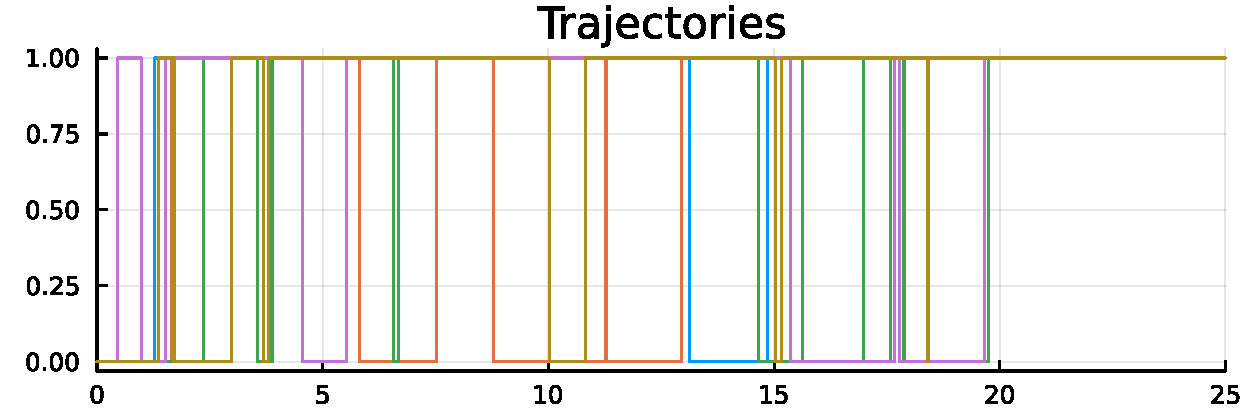
\includegraphics[scale=1.2]{graphics/f6.pdf}
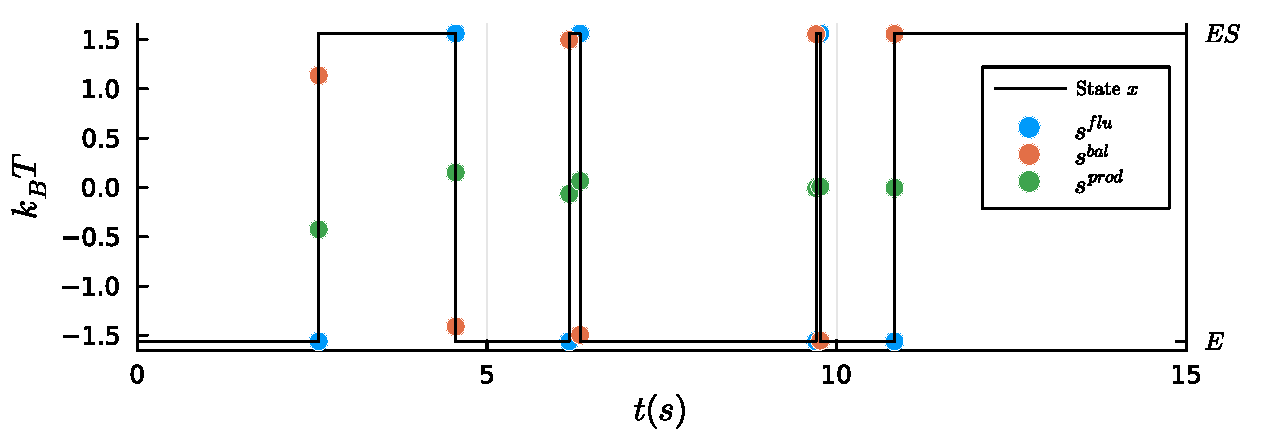
\includegraphics[scale=1.2]{graphics/f8.pdf}
\end{center}
\caption{\justifying Single trajectory of the Markov jump process for the Michaelis-Menten with $k_{1} = 0.5$, $k_{-1} = 0.005$, $k_{2} = 0.1$ and $k_{-2} \approx 0.0$, and entropy exchange/balance/production for that trajectory.}\label{fig transition}
\end{figure}
\begin{figure}
%\vskip-30pt 
\begin{center}
%\includesvg[scale=1.25]{graphics/ST-MM-2.svg}
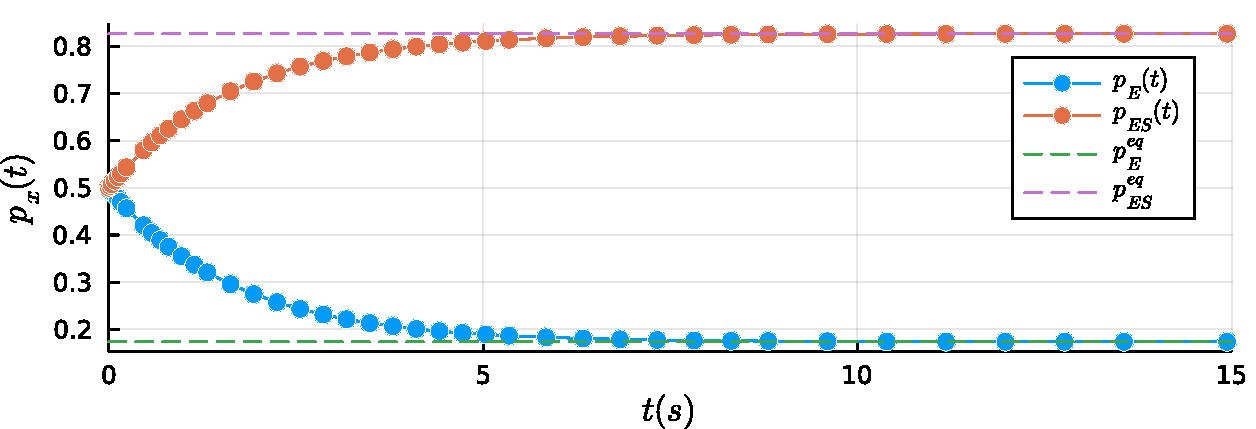
\includegraphics[scale=1.2]{graphics/f1.pdf}
\end{center}
\label{fig 2-state-system}
\caption{\justifying  Time evolution of the probability of the states of the system, $p_E$ and $p_{ES}$, and the probability of the states for the system in equilibrium, $p_E^{eq}$ and $p_{ES}^{eq}$.}
\end{figure}

\begin{figure}
%\vskip-30pt 
\begin{center}
%\includesvg[scale=1.25]{graphics/ST-MM-2.svg}
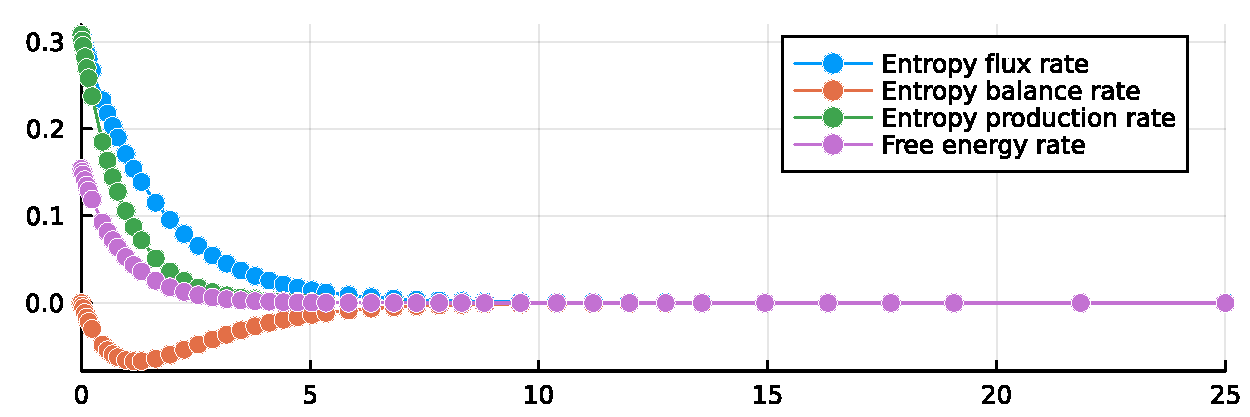
\includegraphics[scale=1.2]{graphics/f2.pdf}
\end{center}
\label{fig 2-state-system}
\caption{\justifying Average entropy flux rate, average entropy production rate, free energy rate and average entropy balance rate.}
\end{figure}

Some conclusions are:
%
\begin{itemize}
\justifying
\item The system relaxes to the equilibrium and, once there, it stabilizes at reservoir properties (e.g. intensive quantities as temperature, chemical potential, etc.);
\item The nonequilibrium free energy of the system is greater than the equilibrium one, thus indicating that work can be exchanged between the system and the reservoir before it gets equilibrated;
\item To sustain the nonequilibrium, work must be applied to the system, which is object of future investigations;
\item The evaluation of the quantities $s^{prod}$, $s^{bal}$, their respective average rates $\dot{S}^{flu}$, $\dot{S}^{prod}$, and $\dot{S}^{bal}$ is only possible because of the numerical solution of \eqref{eq CME}, which is hard to solve for systems with large number of particles. The conventional approach is to use Gillespie algorithm to obtain an ensemble of trajectories;
\item Future explorations are needed to compare the results of the entropies evaluated with the ensemble of trajectories and the numerical integration of \eqref{eq CME}.
\end{itemize}


\end{block}
\end{column}

\separatorcolumn
\end{columns}
 \end{frame}
\end{document}
